\documentclass[runningheads]{llncs}

\usepackage{graphicx}
\usepackage{fontspec}
\usepackage{unicode-math}
\usepackage[Latin,Greek]{ucharclasses}
\usepackage{amsmath}
\usepackage{proof}
\usepackage{bigfoot}
\usepackage{subcaption}
\usepackage[backend=biber]{biblatex}
\addbibresource{references.bib}
\usepackage{listings}
\lstset{
  basicstyle=\ttfamily,
  mathescape
}

\newfontfamily\substitutefont{CMU Serif}
\setTransitionsForGreek{\begingroup\substitutefont}{\endgroup}

% chktex-file 36 
% chktex-file 12

\subtitle{Everybody's Got To Be Somewhere$^{\text{\cite{codebruijn}}}$}
\title{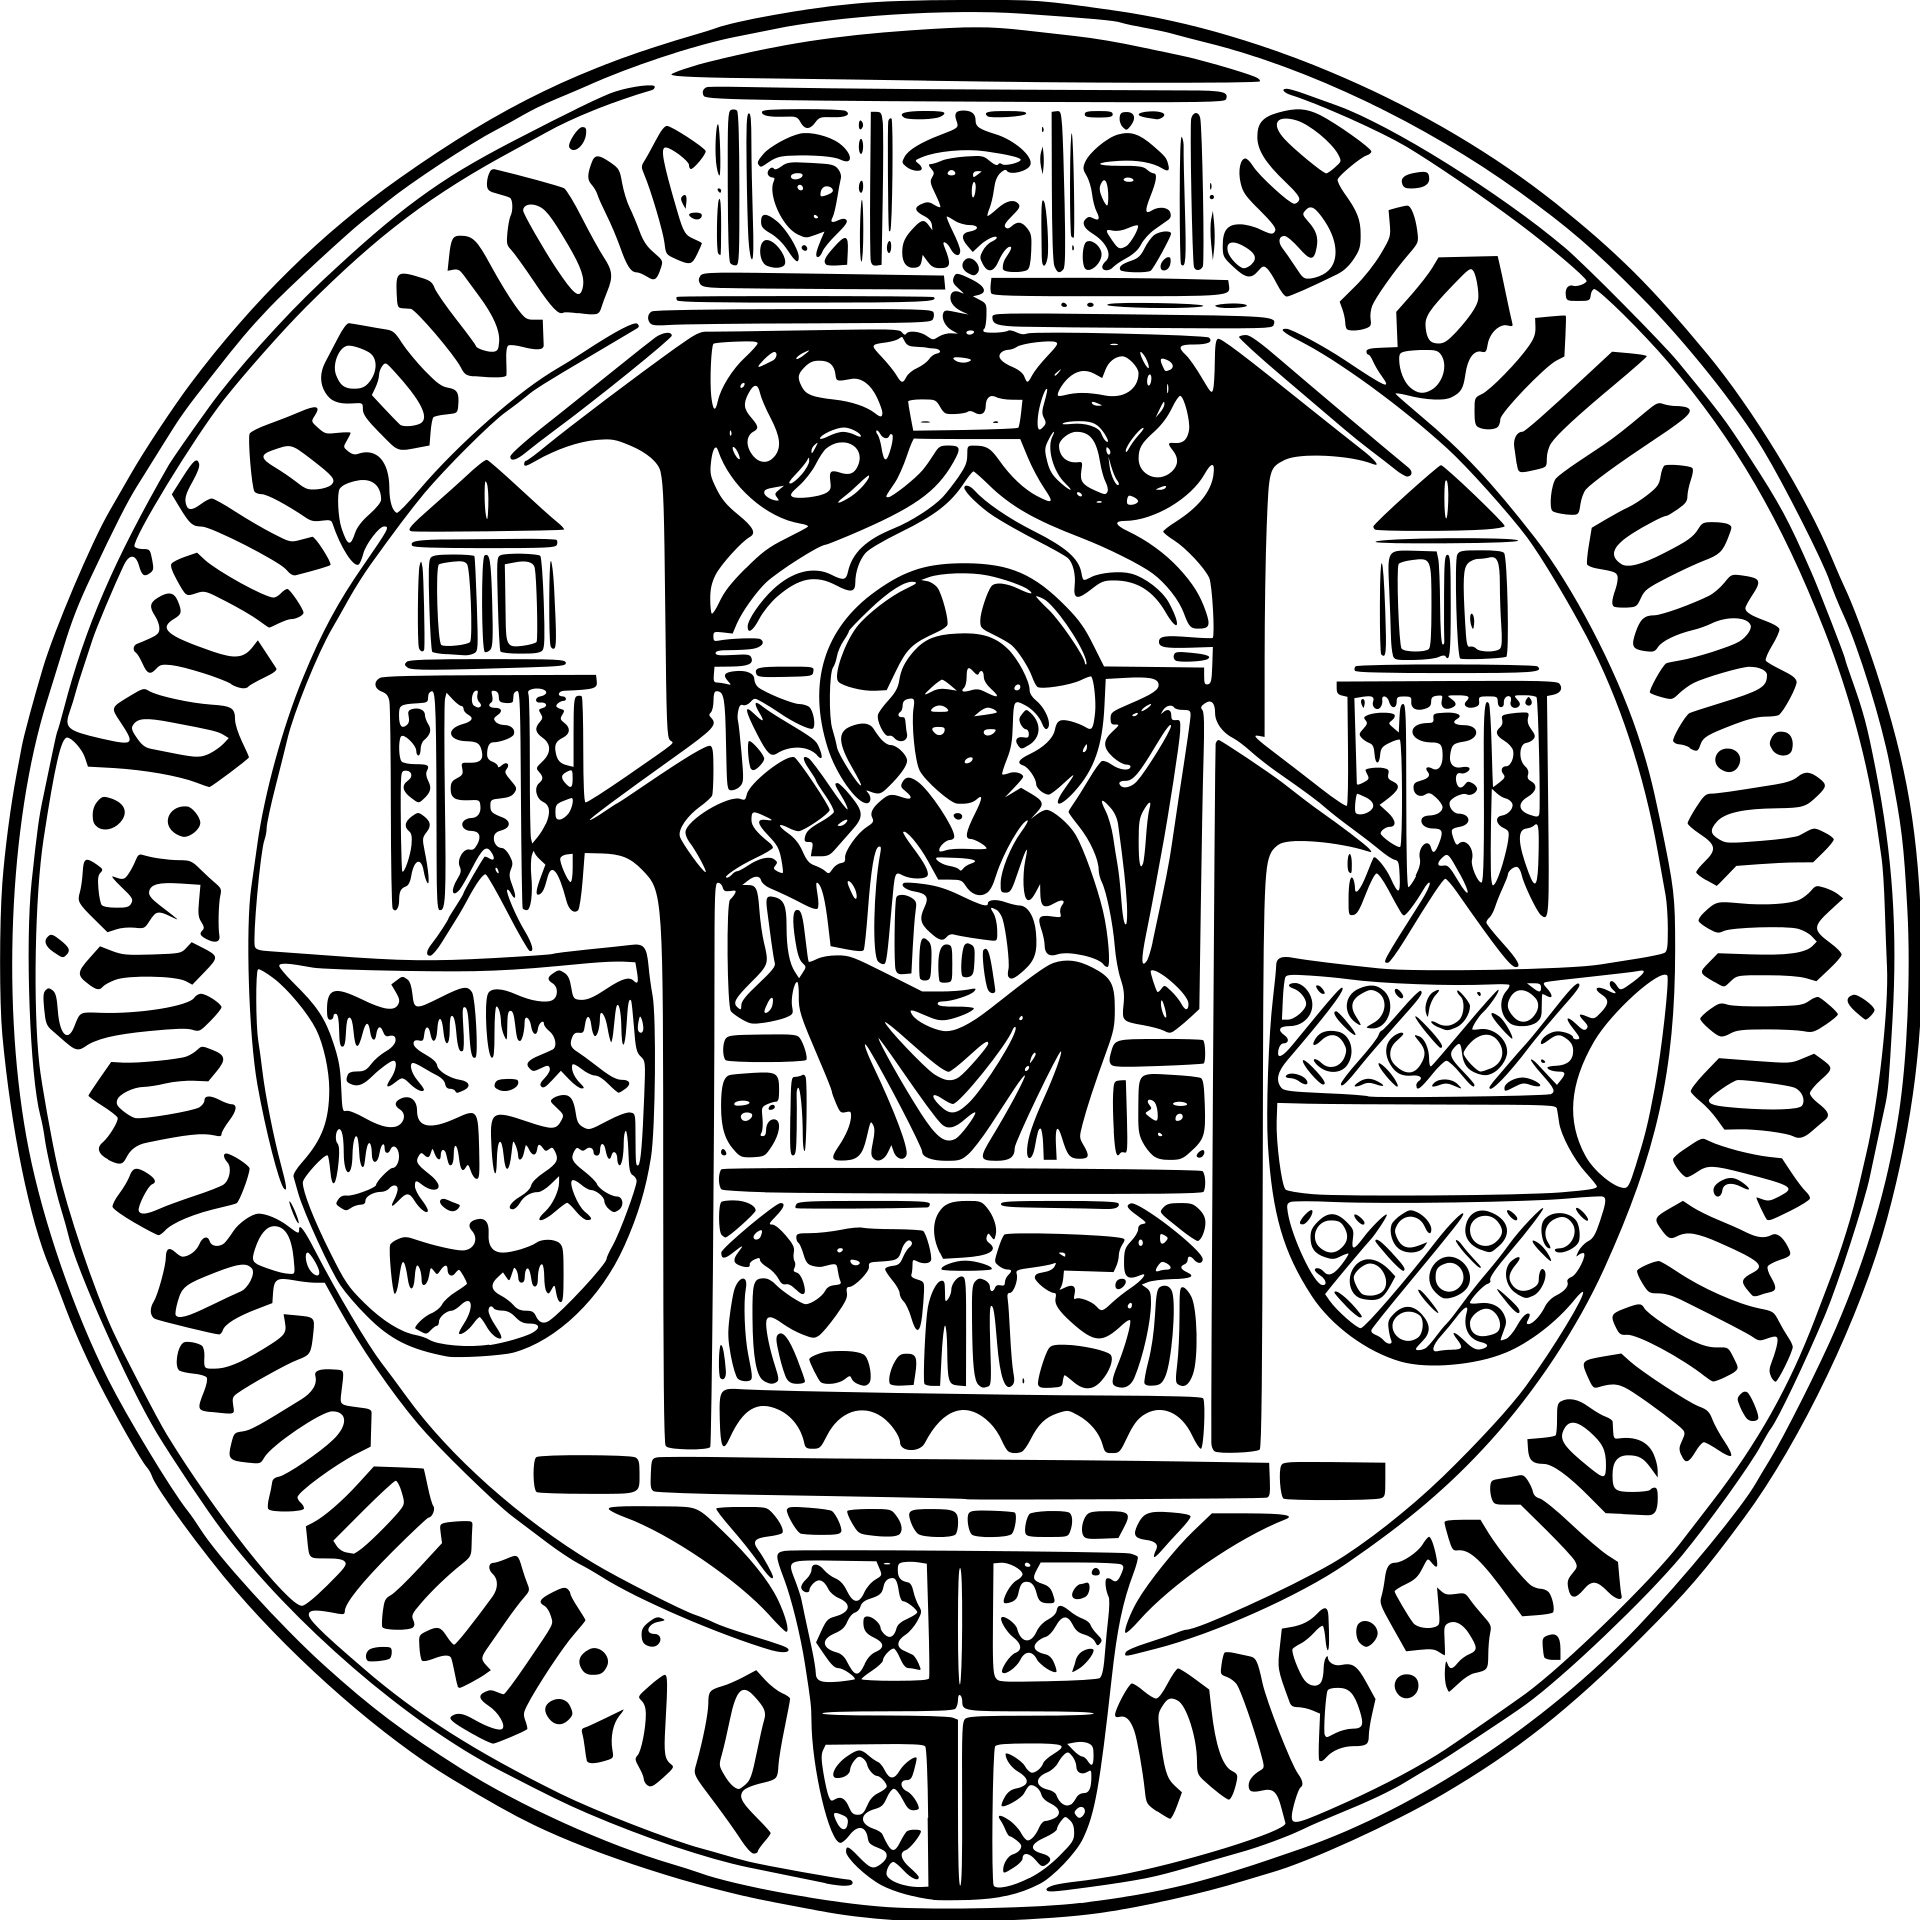
\includegraphics[width=0.4\textwidth]{seal.png}~\\[1cm] From Debruijn to co-Debruijn using Category Theory}
\subtitle{Everybody's Got To Be Somewhere$^{\text{\cite{codebruijn}}}$}
\titlerunning{Elaboration on co-Debruijn}
\institute{Chair of Programming Languages, University of Freiburg \\
  \email{weidner@cs.uni-freiburg.de}}
\author{Marius Weidner}

\begin{document}

\let\oldaddcontentsline\addcontentsline{}
\def\addcontentsline#1#2#3{}
\maketitle
\def\addcontentsline#1#2#3{\oldaddcontentsline{#1}{#2}{#3}}

\begin{abstract}
  We explore the connection between De Bruijn indices used for variable representation in an intrinsically scoped syntax and the adoption of co-De Bruijn representation. 
  To comprehend the duality between De Bruijn and co-De Bruijn, we will look into the categorical concepts underpinning scopes, binders, and intrinsically scoped syntaxes in general. 
  Lastly, we will address challenges encountered in expressing these concepts and investigate the practical application of co-De Bruijn to specific syntaxes within theorem proving contexts.
\end{abstract}

\setcounter{tocdepth}{2}
\tableofcontents
\newpage

\section{Scopes and Binders Categorically}
\subsection{The Category of Scopes}
\subsection{Intrinsically Scoped De Bruijn Syntax}

\section{From De Bruijn to co-De Bruijn}
\subsection{The Slice Category of Scopes}
\subsection{A Monad over Sets Indexed by Scopes}
\subsection{The Notion of Relevant Pairs}
\subsection{Intrinsically Scoped co-De Bruijn Syntax}

\section{Proof Assistants and co-De Bruijn}
\subsection{A Simple co-De Bruijn Syntax in Agda}
\subsection{A Universe of Metasyntaxes with Binding}

\section{Tell them what you have told them}

\printbibliography{}

\end{document}